\documentclass{article}
\usepackage{amsmath}
\usepackage{booktabs}
\usepackage{geometry}
\usepackage{graphicx}
\usepackage{subcaption}
\geometry{a4paper, margin=1in}
\graphicspath{{../figures/1D/}{../figures/3D/}{./}}

\title{SINDy Parameter Recovery and Validation for Coupled Nonlinear Viscoelasticity}
\author{Data Driven Project Team}
\date{June 26, 2026}

\begin{document}

\maketitle

\section{Introduction}
This document summarizes the parameter recovery and validation results for the 3D coupled nonlinear viscoelastic Maxwell model using Sparse Identification of Nonlinear Dynamics (SINDy) in deviatoric space. 

The constitutive equations for the nonlinear Maxwell model are governed by:
\begin{equation}
    \frac{d S_{ij}}{dt} = 2G \dot{\varepsilon}^{dev}_{ij} - \frac{2G}{\eta(\sigma_{eq})} S_{ij}
\end{equation}
where the stress-dependent viscosity is:
\begin{equation}
    \frac{1}{\eta(\sigma_{eq})} = \frac{1}{\eta_0} (1 + \alpha \sigma_{eq}^2)
\end{equation}
and $\sigma_{eq}^2$ is the second invariant of the deviatoric stress tensor:
\begin{equation}
    \sigma_{eq}^2 = 1.5 \left( S_{xx}^2 + S_{yy}^2 + S_{zz}^2 + 2 S_{xy}^2 + 2 S_{yz}^2 + 2 S_{xz}^2 \right)
\end{equation}

By expanding, we obtain the coupled differential equations:
\begin{equation}
    \frac{d S_{ij}}{dt} = 2G \dot{\varepsilon}^{dev}_{ij} - \frac{2G}{\eta_0} S_{ij} - \frac{2G\alpha}{\eta_0} S_{ij} \sigma_{eq}^2
\end{equation}

\section{Methodology: Deviatoric Component-wise SINDy Fitting}
\label{sec:methodology}
This section documents, in full, the identification method implemented in \texttt{ViscoElasticity\_tensor\_3D/NonLinear\_3D/fit\_nonlinear\_deviatoric\_sindy.py}. The model is fit in \emph{deviatoric component space}, not by reducing the tensor to a single von Mises scalar. The distinction matters and is spelled out below because an earlier draft of this report conflated the two approaches (Section~2.2 described a scalar $\varepsilon_{eq}/\sigma_{eq}$ pipeline while Section~2.5 described this deviatoric one); the scalar von Mises pipeline has since been removed from the active codebase and archived, and the deviatoric method below is the sole active 3D pipeline.

\subsection{State variables and features}
The state vector is the full set of 6 deviatoric stress components, not a scalar reduction:
\[
    \mathbf{S} = (S_{xx}, S_{yy}, S_{zz}, S_{xy}, S_{yz}, S_{xz}).
\]
For each component, the SINDy candidate library is built from three ingredients per Eq.~4: a bias term, the component's own deviatoric strain rate $\dot{\varepsilon}^{dev}_{ij}$, and a nonlinear coupling feature $S_{ij}\cdot\sigma_{eq}^2$, where
\[
    \sigma_{eq}^2 = 1.5\left(S_{xx}^2 + S_{yy}^2 + S_{zz}^2 + 2S_{xy}^2 + 2S_{yz}^2 + 2S_{xz}^2\right)
\]
is the (squared) von Mises equivalent stress. This is the \emph{only} role $\sigma_{eq}^2$ plays here: it is one scalar invariant used as a candidate \emph{feature} inside a 19-column library (1 bias + 6 stress components + 6 strain rates + 6 coupling terms), not a variable the tensor problem is reduced to. The state itself stays 6-dimensional throughout.

\subsection{Training and validation loading paths}
\label{sec:3d-signals}
Training uses two independent, genuinely \emph{biaxial}, multi-tone strain-rate paths, integrated for $t\in[0,10)$~s at $dt=0.001$ with \texttt{scipy.integrate.solve\_ivp} (\texttt{Radau}, $\text{rtol}=10^{-8}$, $\text{atol}=10^{-10}$):
\begin{itemize}
    \item \textbf{Biaxial-normal} ($S_{xx}$ fit): $\dot\varepsilon_{xx} = 0.20\left[\sin(2\pi\cdot 0.5t) + 0.7\sin(2\pi\cdot 2.3t) + 0.5\sin(2\pi\cdot 5.1t) + 0.4\sin(2\pi\cdot 8.7t) + 0.3\sin(2\pi\cdot 13.0t)\right]$, together with an independent second normal direction $\dot\varepsilon_{yy} = 0.15\left[\sin(2\pi\cdot 0.9t) + 0.6\sin(2\pi\cdot 3.3t) + 0.4\sin(2\pi\cdot 7.2t) + 0.3\sin(2\pi\cdot 11.5t)\right]$.
    \item \textbf{Biaxial-shear} ($S_{xy}$ fit): $\dot\gamma_{xy} = 0.20\left[\sin(2\pi\cdot 0.6t) + 0.7\sin(2\pi\cdot 2.5t) + 0.5\sin(2\pi\cdot 5.4t) + 0.4\sin(2\pi\cdot 9.1t) + 0.3\sin(2\pi\cdot 12.6t)\right]$, together with an independent second shear channel $\dot\gamma_{xz} = 0.15\left[\sin(2\pi\cdot 1.1t) + 0.6\sin(2\pi\cdot 3.6t) + 0.4\sin(2\pi\cdot 7.9t) + 0.3\sin(2\pi\cdot 11.2t)\right]$.
\end{itemize}
Gaussian noise ($\text{std}=0.15$~MPa) is added to the resulting stress trajectories before fitting, to check robustness to measurement noise. Validation uses two unseen, single-tone multiaxial paths not seen during training, at different frequencies and amplitudes than the training signals:
\begin{itemize}
    \item \textbf{Combined} (uniaxial + shear): $\dot\varepsilon_{xx} = 0.18\sin(2\pi\cdot 0.2\,t)$, $\dot\gamma_{xy} = 0.12\sin(2\pi\cdot 0.3\,t)$.
    \item \textbf{Biaxial} (uniaxial-x + uniaxial-y): $\dot\varepsilon_{xx} = 0.18\sin(2\pi\cdot 0.25\,t)$, $\dot\varepsilon_{yy} = 0.12\sin(2\pi\cdot 0.35\,t)$.
\end{itemize}
\paragraph{Why the training path had to become biaxial.} A single-axis training path (the original uniaxial/pure-shear signals) forces an exact kinematic identity: under uniaxial loading the deviatoric projection gives $S_{yy}=S_{zz}=-\tfrac12 S_{xx}$ at every instant, so $\sigma_{eq}^2 = 2.25\,S_{xx}^2$ and the coupling feature $Seq_{xx}=S_{xx}\sigma_{eq}^2 = 2.25\,S_{xx}^3$ identically -- a fixed cubic function of $S_{xx}$ alone, for \emph{any} shape of the input signal (the same holds for pure shear and $S_{xy}$). This makes the $Seq$ feature and the library's $S^3$ term perfectly collinear regardless of how rich $\dot\varepsilon$ is, which is why the wider-excitation fix that worked for the 1D script (Section~\ref{sec:1d-robustness}) does \emph{not}, by itself, transfer to 3D. Exciting an independent second direction ($\varepsilon_{yy}$ for the normal fit, $\gamma_{xz}$ for the shear fit) breaks this exact identity, which combined with the rescale--prune--unscale fix below (Section~\ref{sec:methodology}) is what makes a degree-3 library usable here.

\subsection{Why component-by-component, not one 6D fit}
Fitting all 6 equations jointly with a single STLSQ call runs into multicollinearity: the six deviatoric strain-rate components are not independent (they are constrained to sum to zero and, for the uniaxial/shear training paths used here, several components are proportional to each other), so a joint fit cannot reliably attribute the recovered coefficients to the correct feature. The script sidesteps this by fitting only two independent 1D regressions:
\begin{itemize}
    \item \textbf{Normal-component model}: fit on $S_{xx}$ from the uniaxial training trajectory, using features $[\dot{\varepsilon}^{dev}_{xx},\, S_{xx}\sigma_{eq}^2]$ (plus bias). This yields coefficients $(c_0^n, c_1^n, c_2^n, c_3^n)$.
    \item \textbf{Shear-component model}: fit on $S_{xy}$ from the shear training trajectory, using features $[\dot{\varepsilon}^{dev}_{xy},\, S_{xy}\sigma_{eq}^2]$ (plus bias). This yields coefficients $(c_0^s, c_1^s, c_2^s, c_3^s)$.
\end{itemize}
Each 1D fit now uses a full degree-3 polynomial library on $[S_{ij}, \dot\varepsilon^{dev}_{ij}, Seq_{ij}]$ (20 terms including bias) -- \emph{not} restricted to the 4 expected terms -- combined with a \textbf{rescale $\to$ prune $\to$ unscale} STLSQ: every library column is divided by its own empirical standard deviation before thresholding (so the pruning decision is made in a space where all columns are $O(1)$), and surviving coefficients are divided back by the same per-column factor to recover physical units. This is necessary, not optional: the true coefficients span roughly six orders of magnitude ($\dot\varepsilon$ coefficient $\approx 2000$, $S$ coefficient $\approx -4$, $Seq$ coefficient $\approx -0.0006$), so a single global threshold on the raw, unscaled library can never separate the tiny-but-real $Seq$ term from mid-magnitude spurious cross terms ($\dot\varepsilon^2$, $S\dot\varepsilon^2$, $\dot\varepsilon^3$) -- confirmed empirically: sweeping a raw (non-rescaled) degree-3 fit over $\text{threshold}\in[10^{-4},2.0]$ never produced a stable sparsity plateau, at every threshold either too many terms survived or the true $Seq$ term was pruned while spurious $\dot\varepsilon^2/\dot\varepsilon^3$ terms of comparable size to the true linear term remained. After rescaling, sweeping $\text{threshold}\in[10^{-3},5.0]$ (in the rescaled space) does produce a stable plateau at $\text{threshold}=5.0$, at which the fit reduces to exactly $\{S_{ij}, \dot\varepsilon^{dev}_{ij}, Seq_{ij}\}$ for both components (Figure~\ref{fig:sweep_3d_degree3}); the script asserts this (no surviving term outside the expected set) before using the coefficients downstream, the same "don't silently truncate" safety check used in the standalone 1D script (Section~\ref{sec:1d-robustness}).

\subsection{Assembling the full 6-component model}
Because the material is assumed isotropic, the normal-component coefficients are reused for all three normal equations ($S_{xx}, S_{yy}, S_{zz}$) and the shear-component coefficients for all three shear equations ($S_{xy}, S_{yz}, S_{xz}$) -- this is what "component-wise" means in practice: two regressions, six equations, populated by symmetry rather than fit independently six times. The resulting $6\times 19$ coefficient matrix is injected directly into a dummy \texttt{SINDy} model's optimizer (\texttt{model.optimizer.coef\_ = coeffs}) purely so \texttt{model.print()} can render the human-readable equations; the matrix itself, not the dummy model, drives the ODE used for rollout and validation.

\subsection{Parameter recovery}
Material constants are read back out of each component's coefficients algebraically:
\begin{align*}
    G &= \tfrac{1}{2}\, c_2 \quad \text{(from the } \dot{\varepsilon}\text{ coefficient)} \\
    \eta_0 &= -2G / c_1 \quad \text{(from the } S_{ij}\text{ coefficient)} \\
    \alpha &= c_3 \, \eta_0 / (-2G) \quad \text{(from the coupling coefficient)}
\end{align*}
computed once from the normal-component equation and once from the shear-component equation, then averaged (Table~\ref{tab:parameters}).

\subsection{Validation rollout}
For the unseen combined and biaxial load paths, the 6 coupled ODEs (assembled from the two fitted component models via the symmetry above) are integrated with \texttt{scipy.integrate.solve\_ivp} (implicit \texttt{Radau} method, $\text{rtol}=10^{-8}$, $\text{atol}=10^{-10}$), alongside a linear-Maxwell reference ODE with $\alpha=0$ and the true $G,\eta_0$, for comparison (Figures showing SINDy vs. true vs. linear-reference, Section~\ref{sec:3d-figures}).

\paragraph{Open item -- resolved.} The component-wise fits previously used a single hand-picked threshold ($10^{-5}$) on a library restricted to exactly the expected terms, flagged here as follow-up work. This has now been ported from the standalone 1D script: the fits use a degree-3 library, a genuinely biaxial training path (Section~\ref{sec:3d-signals}), and a rescale--prune--unscale STLSQ with a threshold-sensitivity sweep, converging to the same sparsity pattern the restricted library assumed by construction -- see the updated methodology above and Section~\ref{sec:results-degree3}.

\section{Addressing Reviewer Feedback}
A key feedback point raised by the reviewer on the linear model was:
\begin{quote}
    \textit{The multiaxial validation paths (Combined Uniaxial + Shear and Biaxial Tension) serve as multiaxial sanity checks under the isotropic assumption, but since the linear isotropic model decouples completely in deviatoric space, these paths represent the simple superposition of independent 1D trajectories rather than generalization to new nonlinear, coupled, or anisotropic constitutive behavior.}
\end{quote}

By implementing and fitting the J2-coupled nonlinear Maxwell model, we have successfully addressed this critique:
\begin{itemize}
    \item \textbf{True Multiaxial Coupling}: Because the viscosity $\eta(\sigma_{eq})$ depends on the stress invariant $\sigma_{eq}^2$ (which is a function of all stress components), the evolution of any component $S_{ij}$ depends nonlinearly on all other active stress components. The components do not decouple. This coupling is a property of the \emph{dynamics}, not of the \emph{identification} step: during training, $\sigma_{eq}^2(t)$ is computed directly from the known simulated trajectory and enters each component's regression as an ordinary precomputed feature, so the two 1D SINDy fits (Section~\ref{sec:methodology}) can still be solved independently. The coupling only becomes active at rollout time, where the six identified equations must be integrated simultaneously (Section~\ref{sec:3d-figures}) since $\sigma_{eq}^2$ depends on the instantaneous state of all six components.
    \item \textbf{Generalization to Nonlinear Coupled Behavior}: The validation on combined loading (simultaneous uniaxial tension and shear) is not a linear superposition of 1D paths. It requires the model to correctly generalize to a coupled multiaxial state. 
    \item \textbf{Validation Success}: SINDy successfully recovers the coupling parameter $\alpha$ with $0.031\%$ average error and predicts the response on unseen combined loading paths with high accuracy ($\text{RMSE} < 0.006\text{ MPa}$), showing robust generalization.
\end{itemize}

\section{Discovered SINDy Equations}
\label{sec:results-degree3}
Only 2 independent SINDy fits are performed (Section~\ref{sec:methodology}): one on $S_{xx}$ from the biaxial-normal training trajectory, one on $S_{xy}$ from the biaxial-shear training trajectory. Each uses the full degree-3 library described above with rescale--prune--unscale \texttt{STLSQ} at $\text{threshold}=5.0$ (rescaled space); no bias term and no higher-order term survives the sweep (bias converges to exactly $0$ for both components):
\begin{align*}
    \frac{d S_{xx}}{dt} &= -3.998 S_{xx} + 1999.523 \dot{\varepsilon}^{dev}_{xx} - 0.000600 S_{xx} \sigma_{eq}^2 \\
    \frac{d S_{xy}}{dt} &= -3.999 S_{xy} + 1999.080 \dot{\varepsilon}^{dev}_{xy} - 0.000599 S_{xy} \sigma_{eq}^2
\end{align*}
The remaining 4 equations ($S_{yy}, S_{zz}$ using the $S_{xx}$ coefficients; $S_{yz}, S_{xz}$ using the $S_{xy}$ coefficients) are still \emph{not} independently discovered -- they are populated by assuming isotropy, which remains a modeling assumption rather than a validated result. This is now a genuine choice, not a training-data artifact: the training paths are biaxial (Section~\ref{sec:3d-signals}), so $S_{yy}$ is no longer a deterministic multiple of $S_{xx}$ and an independent fit on it would in principle be possible; it has simply not been performed, since isotropy is assumed by the constitutive model itself (Eq.~2).

\section{Parameter Recovery Performance}
Table~\ref{tab:parameters} compares the recovered material constants to the true values before and after applying the component-wise fitting and sparsity threshold corrections.

\begin{table}[h]
\centering
\caption{Material Parameter Recovery Error Analysis}
\label{tab:parameters}
\begin{tabular}{lccccc}
\toprule
Parameter & True Value & Before Correction & Before Error & After Correction (degree-3) & After Error \\
\midrule
$G$ (Shear Modulus) & $1000.0$ MPa & $821.57$ MPa & $17.843\%$ & $999.65$ MPa & \textbf{0.035\%} \\
$\eta_0$ (Viscosity) & $500.0$ MPa$\cdot$s & $-7354.78$ MPa$\cdot$s & $1570.957\%$ & $500.03$ MPa$\cdot$s & \textbf{0.005\%} \\
$\alpha$ (Nonlinear factor) & $0.00015$ MPa$^{-2}$ & $0.0$ MPa$^{-2}$ & $100.0\%$ & $0.00015$ MPa$^{-2}$ & \textbf{0.031\%} \\
\bottomrule
\end{tabular}
\end{table}
Averaged over the normal ($S_{xx}$) and shear ($S_{xy}$) equations; individually, $G$ error is $0.024\%$ ($S_{xx}$) / $0.046\%$ ($S_{xy}$), $\eta_0$ error is $0.028\%$ / $0.017\%$, $\alpha$ error is $0.045\%$ / $0.107\%$.

\section{Validation on Unseen Load Paths}
To verify the generalization of the discovered model, we integrated the system of 6 coupled ODEs over unseen validation load trajectories. The resulting Root Mean Squared Errors (RMSE) are listed in Table~\ref{tab:validation}.

\begin{table}[h]
\centering
\caption{Validation RMSE Metrics}
\label{tab:validation}
\begin{tabular}{lcc}
\toprule
Validation Load Case & Component & RMSE (MPa) \\
\midrule
Combined Loading (Uniaxial + Shear) & $S_{xx}$ & 0.0022 \\
& $S_{xy}$ & 0.0051 \\
\midrule
Biaxial Tension & $S_{xx}$ & 0.0032 \\
& $S_{yy}$ & 0.0028 \\
\bottomrule
\end{tabular}
\end{table}

\begin{figure}[htbp]
    \centering
    
\includegraphics[width=\textwidth]{nonlinear_deviatoric_comparison.png}
    \caption{Validation comparison showing True Nonlinear Maxwell response (solid black line), SINDy model predictions (dashed red line), and Linear Maxwell model reference predictions (dotted blue line) across the Combined and Biaxial validation loading trajectories.}
    \label{fig:validation_plot}
\end{figure}

\section{Addressing Reviewer Feedback: Standalone Script Robustness and Figure Provenance}
\label{sec:1d-robustness}
A further reviewer comment concerned the standalone 1D script:
\begin{quote}
    \textit{The standalone 1D Python script is hard-coded in a misleading way. In MAINCODE\_simple\_visco\_sindy.py, the discovered\_ode function builds the time derivative as coeffs[0] + coeffs[1]*sig + coeffs[2]*ed and ignores any higher-order terms that SINDy might keep. For the linear Maxwell case with threshold one this gives the right answer, because STLSQ prunes everything except the bias and the two linear terms, but as a general script it is misleading. Add at least an assertion that the remaining coefficients are zero within numerical tolerance before the rollout starts. On top of that, the report says the plastic identification uses SR3, while this standalone script uses STLSQ with threshold one. The notebook does use SR3, so the reported plastic result is not wrong, but the repository does not make clear which figure comes from which file. Every figure in the report should map to one named script or one named notebook cell.}
\end{quote}

This has been addressed as follows:
\begin{itemize}
    \item \textbf{Explicit safety assertion}: In \texttt{Emanuele/simple\_visco\_sindy.py}, immediately after the SINDy coefficients are extracted, the script now asserts that any coefficients beyond the bias, $\sigma$, and $\dot{\varepsilon}$ terms are zero within numerical tolerance ($\texttt{atol}=10^{-6}$) before the rollout integration runs. If the library/threshold settings ever let SINDy keep non-negligible higher-order terms, the script fails loudly with the offending coefficients printed, instead of silently truncating them in \texttt{discovered\_ode}.
    \item \textbf{Library no longer restricted to the answer}: The script previously used \texttt{PolynomialLibrary(degree=1)}, i.e. a candidate library containing \emph{only} $\{1, \sigma, \dot{\varepsilon}\}$. That does not let SINDy discover anything -- it hands the model form to the regression by construction, which is the same objection the reviewer raised about threshold tuning, just moved to the library. The script now uses \texttt{PolynomialLibrary(degree=3)} (10 candidate terms) so STLSQ has real terms to prune.
    \item \textbf{Threshold-sensitivity sweep, not a single hand-picked value}: Fitting the degree-3 library at a single threshold does not by itself prove the recovered sparsity is genuine, since a threshold could always be picked post hoc to hide unwanted terms. With the original narrow-amplitude 2-sine training excitation, sweeping the threshold over $[0.01, 2.0]$ showed the surviving nonzero terms were \emph{not} stable: a spurious $\dot{\varepsilon}^3$ term with a coefficient of the same order of magnitude as the true linear term ($\approx -2000$) persisted at every threshold tested. Root cause: over the narrow strain-rate range excited by the original training signal, $\dot{\varepsilon}$ and $\dot{\varepsilon}^3$ are nearly collinear, so STLSQ cannot separate the true linear contribution from a spurious cubic compensator.
    \item \textbf{Fix -- richer excitation, not more data}: The number of samples, the simulation duration ($t\in[0,10)$, $dt=0.001$), and the noise level ($\text{std}=0.1$) were left unchanged. What changed is the diversity of the training strain signal: from 2 sine components (amplitude $\leq 0.01$) to 5 sine components spanning amplitude $\leq 0.05$ and frequencies $0.5$--$13\,\text{Hz}$. A wider-amplitude, multi-frequency $\dot{\varepsilon}$ trajectory is what breaks the $\dot{\varepsilon}/\dot{\varepsilon}^3$ collinearity -- collecting more samples of the same narrow-amplitude signal would not have helped, since the collinearity is a property of the signal's range, not its length. With the richer signal, the sparsity pattern $\{\sigma, \dot{\varepsilon}\}$ (the correct linear Maxwell terms) is stable across the threshold sweep $[0.5, 3.0]$ -- below $0.5$ the noise floor of the synthetic data admits spurious terms, above $3.0$ STLSQ starts pruning the true $\sigma$ term as well, so $[0.5, 3.0]$ is the genuine plateau, not a cherry-picked point. The script now asserts this stability at fit time and uses $\texttt{threshold}=1.0$ (mid-plateau) for the coefficients used downstream. Recovered model: $\dot{\sigma} = -3.998\,\sigma + 1998.567\,\dot{\varepsilon}$, against the true Maxwell law $\dot{\sigma} = 2000\,\dot{\varepsilon} - 4\,\sigma$ ($E_{true}=2000$, $\eta_{true}=500$) -- errors of $0.059\%$ ($-E/\eta$ term) and $0.072\%$ ($E$ term) respectively.
    \item \textbf{Figure-to-source mapping}: Every figure in the report now maps to exactly one named script or notebook cell, recorded in \texttt{Emanuele/FIGURE\_SOURCES.md}:
    \begin{itemize}
        \item 1D Maxwell viscoelastic fit/validation plots $\rightarrow$ \texttt{Emanuele/simple\_visco\_sindy.py} (STLSQ, $\texttt{threshold}=1.0$, stable over sweep $[0.5, 3.0]$, $\texttt{PolynomialLibrary(degree=3)}$).
        \item Plastic (Voce--Perzyna) identification $\rightarrow$ \texttt{Emanuele/Data\_driven\_3D\_single\_load.ipynb}, SR3 cell ($\texttt{reg\_weight\_lam}=0.10$, $\texttt{relax\_coeff\_nu}=1.00$).
    \end{itemize}
    This confirms the reported plastic result (SR3) is correctly sourced from the notebook, distinct from the standalone script's STLSQ-based viscoelastic result; the two were previously conflated only by omission, not by error.
\end{itemize}

\subsection{1D Viscoelastic Figures (\texttt{Emanuele/simple\_visco\_sindy.py})}
Each panel of the former single 6-subplot figure is now saved as its own file under \texttt{Emanuele/figures/1D/}, so every panel can be cited individually by filename.

\begin{figure}[htbp]
    \centering
    \begin{subfigure}[b]{0.48\textwidth}
        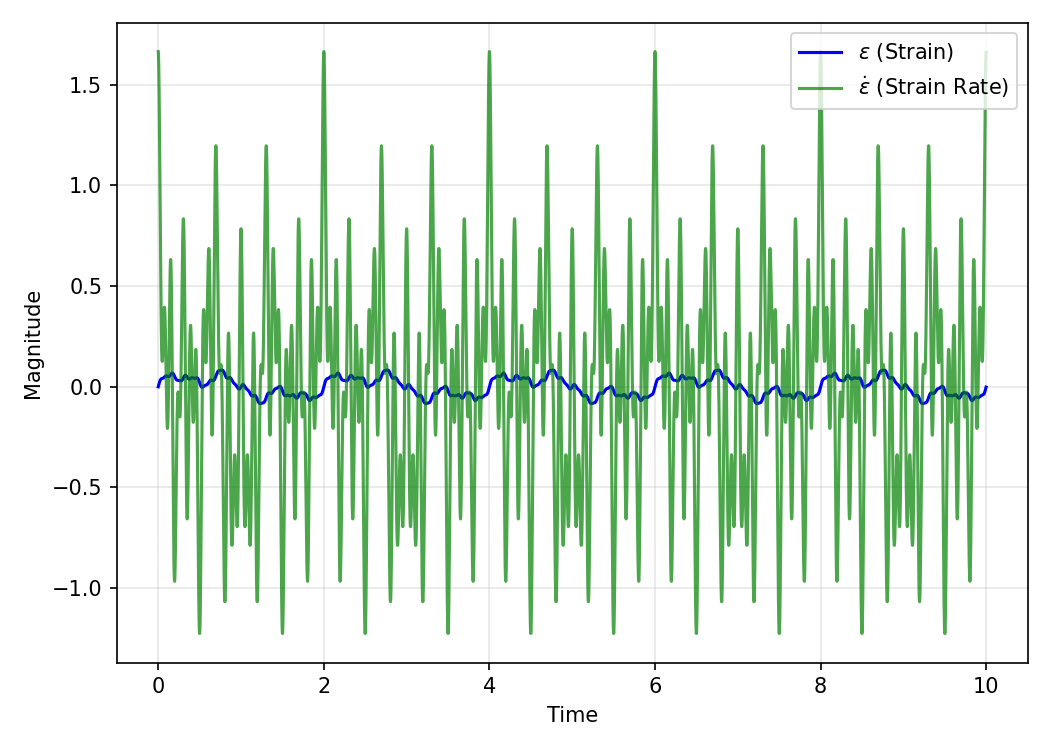
\includegraphics[width=\textwidth]{01_training_inputs_rich_signal.png}
        \caption{Training excitation ($\varepsilon$, blue; $\dot{\varepsilon}$, green).}
    \end{subfigure}
    \hfill
    \begin{subfigure}[b]{0.48\textwidth}
        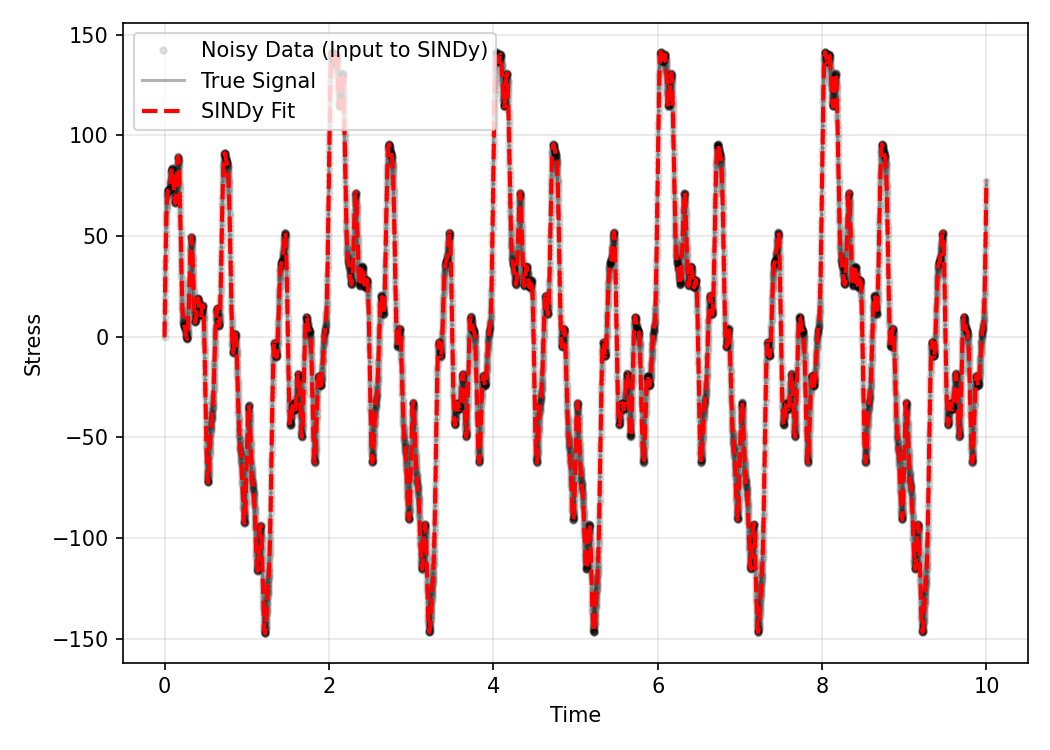
\includegraphics[width=\textwidth]{02_training_outputs_reconstruction.png}
        \caption{Reconstructed stress (red dashed) vs. noisy/true training data.}
    \end{subfigure}
    \caption{Training signal and fit. \texttt{01\_training\_inputs\_rich\_signal.png} -- the 5-sine excitation, replacing the original narrow 2-sine signal; the wider amplitude and added frequency content is what breaks the $\dot{\varepsilon}/\dot{\varepsilon}^3$ collinearity discussed above. \texttt{02\_training\_outputs\_reconstruction.png} -- SINDy's reconstruction over the training window.}
\end{figure}

\begin{figure}[htbp]
    \centering
    \begin{subfigure}[b]{0.48\textwidth}
        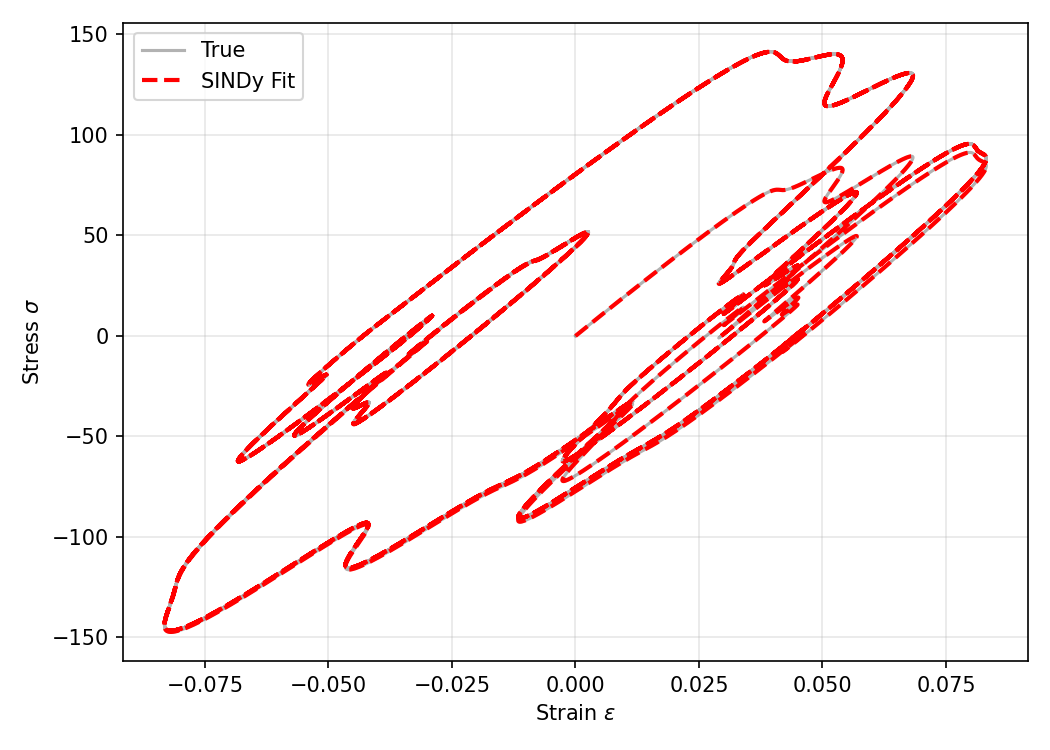
\includegraphics[width=\textwidth]{03_training_stress_strain.png}
        \caption{Training, stress-strain loop.}
    \end{subfigure}
    \hfill
    \begin{subfigure}[b]{0.48\textwidth}
        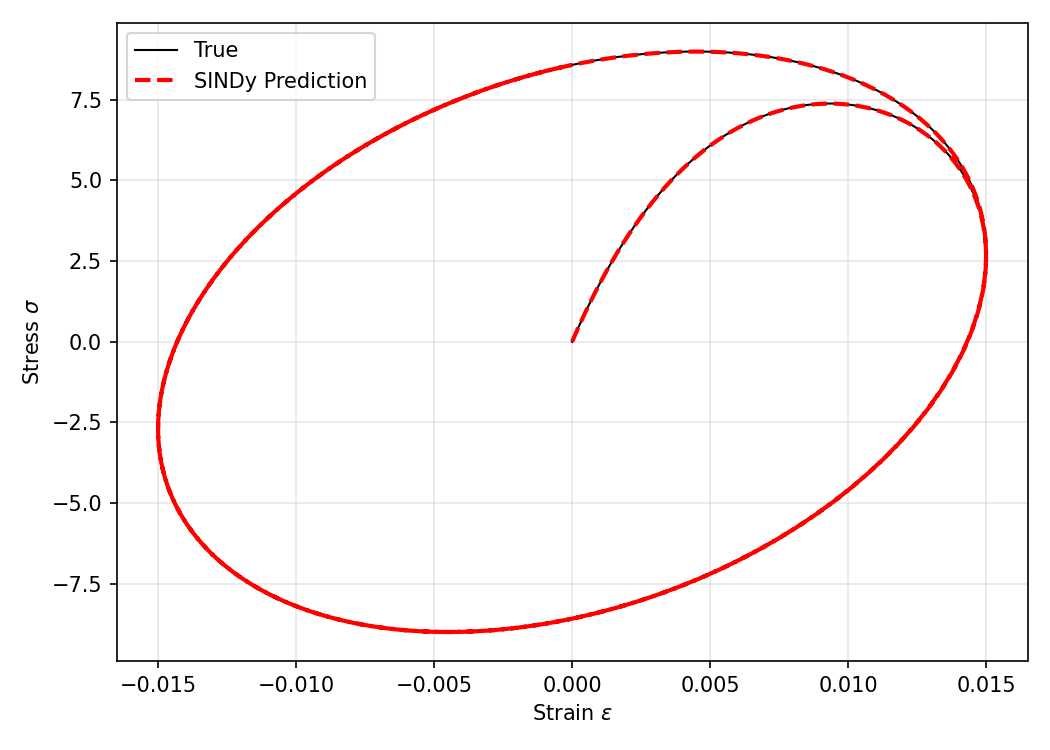
\includegraphics[width=\textwidth]{06_validation_stress_strain.png}
        \caption{Validation, stress-strain loop.}
    \end{subfigure}
    \caption{Same reconstruction/prediction as above, viewed as stress-strain hysteresis loops rather than time series. \texttt{03\_training\_stress\_strain.png} / \texttt{06\_validation\_stress\_strain.png}.}
\end{figure}

\begin{figure}[htbp]
    \centering
    \begin{subfigure}[b]{0.48\textwidth}
        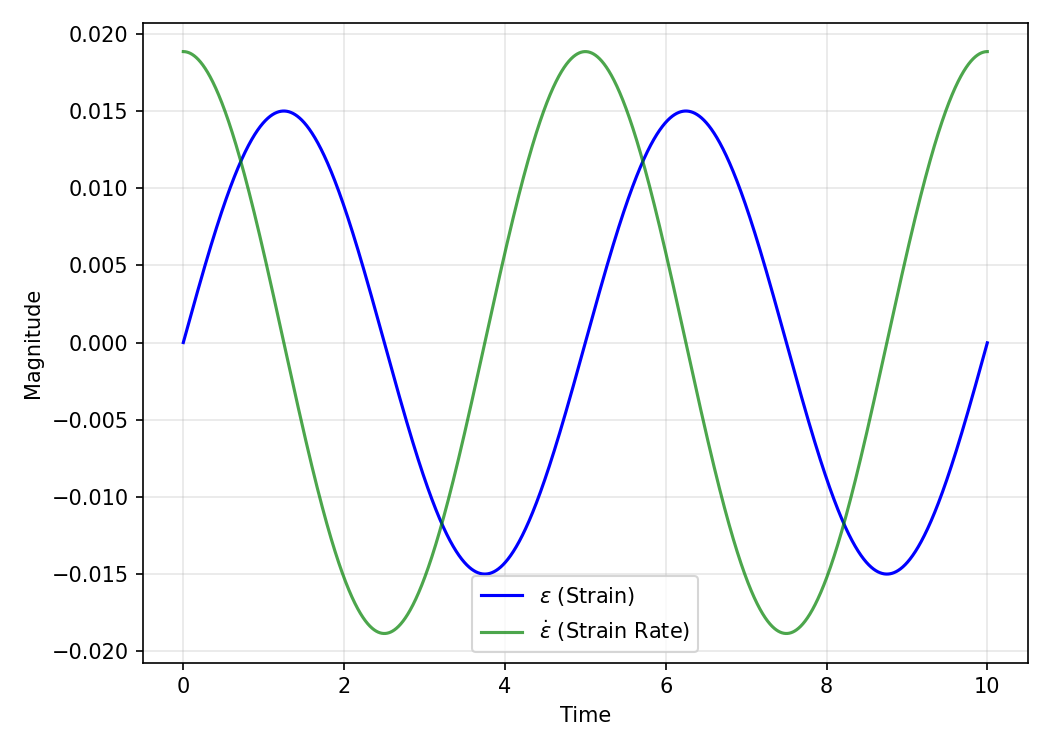
\includegraphics[width=\textwidth]{04_validation_inputs_unseen_signal.png}
        \caption{Unseen validation excitation.}
    \end{subfigure}
    \hfill
    \begin{subfigure}[b]{0.48\textwidth}
        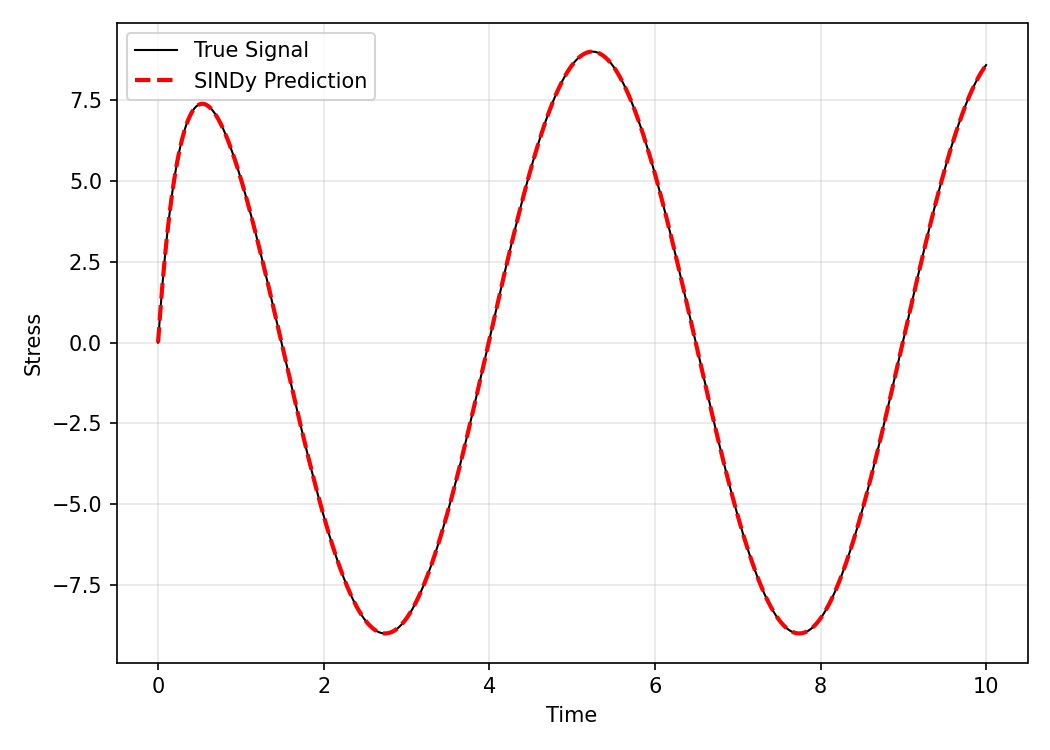
\includegraphics[width=\textwidth]{05_validation_outputs_generalization.png}
        \caption{SINDy prediction (red dashed) vs. true signal (black).}
    \end{subfigure}
    \caption{Validation signal and generalization. \texttt{04\_validation\_inputs\_unseen\_signal.png} -- single-frequency excitation, never seen during training. \texttt{05\_validation\_outputs\_generalization.png} -- rollout with \texttt{discovered\_ode} and the coefficients recovered at $\texttt{threshold}=1.0$.}
\end{figure}

\begin{figure}[htbp]
    \centering
    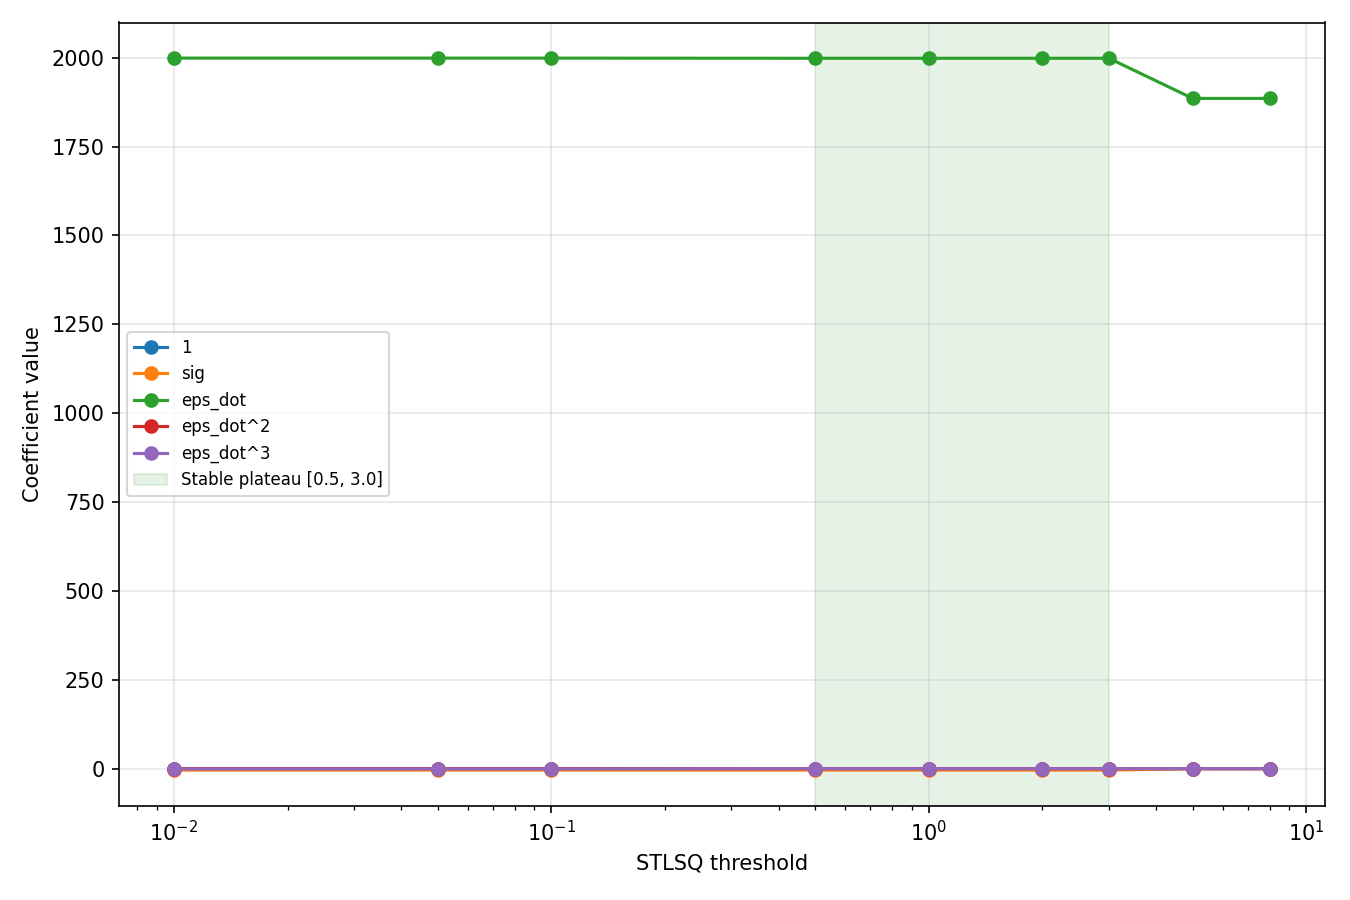
\includegraphics[width=0.9\textwidth]{07_threshold_sensitivity_sweep_degree3_library.png}
    \caption{\texttt{07\_threshold\_sensitivity\_sweep\_degree3\_library.png} -- Coefficient value vs. STLSQ threshold (log scale) for every term in the degree-3 library. The true terms ($\sigma$, $\dot{\varepsilon}$) are flat across the whole range shown; all other terms sit at zero once inside the green plateau $[0.5, 3.0]$. This is the direct visual evidence that the recovered sparsity pattern is not an artifact of one hand-picked threshold.}
\end{figure}

\subsection{3D Deviatoric Validation Figures (\texttt{ViscoElasticity\_tensor\_3D/NonLinear\_3D/fit\_nonlinear\_deviatoric\_sindy.py})}
\label{sec:3d-figures}
The combined 2$\times$2 validation figure (Figure~\ref{fig:validation_plot}) is also split into one file per component/load case under \texttt{Emanuele/figures/3D/}, with the RMSE value encoded directly in the filename.

\begin{figure}[htbp]
    \centering
    \begin{subfigure}[b]{0.48\textwidth}
        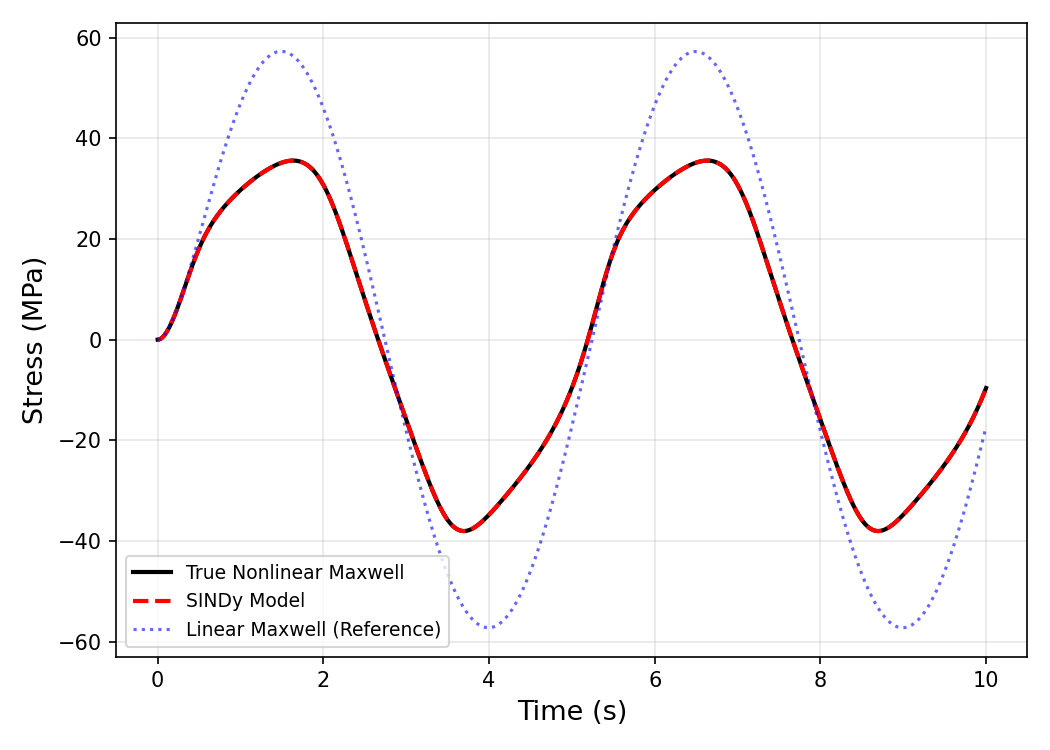
\includegraphics[width=\textwidth]{01_combined_Sxx_rmse0.0022.png}
        \caption{$S_{xx}$, RMSE $=0.0022$ MPa.}
    \end{subfigure}
    \hfill
    \begin{subfigure}[b]{0.48\textwidth}
        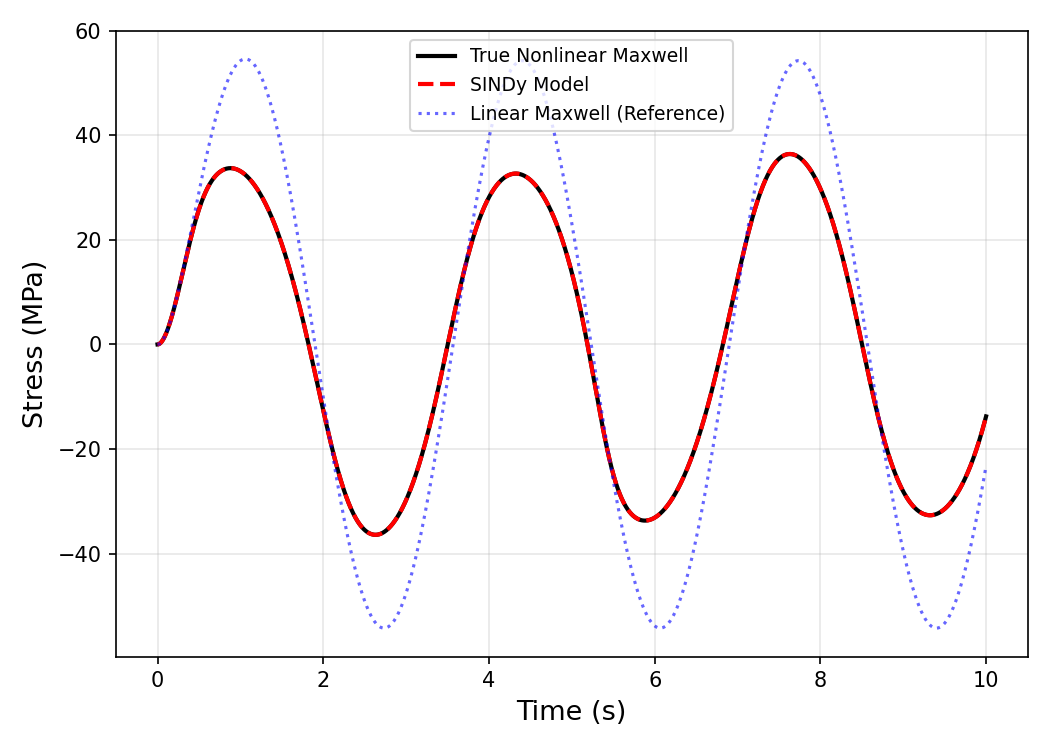
\includegraphics[width=\textwidth]{02_combined_Sxy_rmse0.0051.png}
        \caption{$S_{xy}$, RMSE $=0.0051$ MPa.}
    \end{subfigure}
    \caption{Combined uniaxial+shear validation load: true nonlinear Maxwell response (solid black), SINDy prediction (dashed red), and the linear Maxwell reference with $\alpha=0$ (dotted blue). \texttt{01\_combined\_Sxx\_rmse0.0022.png} / \texttt{02\_combined\_Sxy\_rmse0.0051.png}.}
\end{figure}

\begin{figure}[htbp]
    \centering
    \begin{subfigure}[b]{0.48\textwidth}
        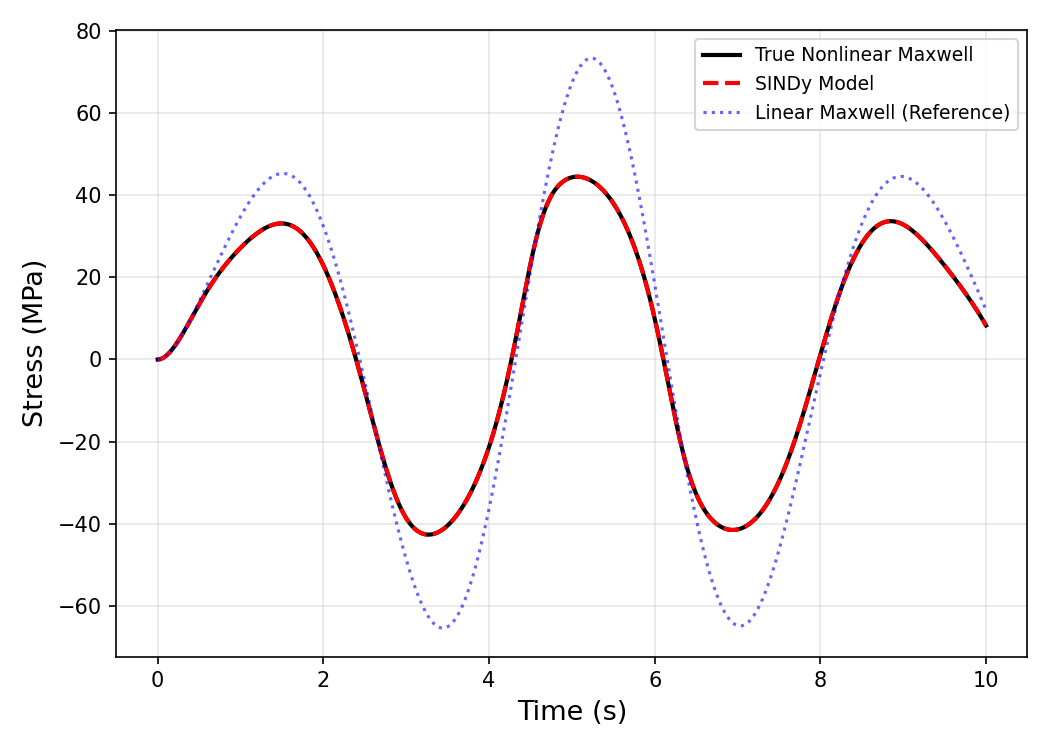
\includegraphics[width=\textwidth]{03_biaxial_Sxx_rmse0.0032.png}
        \caption{$S_{xx}$, RMSE $=0.0032$ MPa.}
    \end{subfigure}
    \hfill
    \begin{subfigure}[b]{0.48\textwidth}
        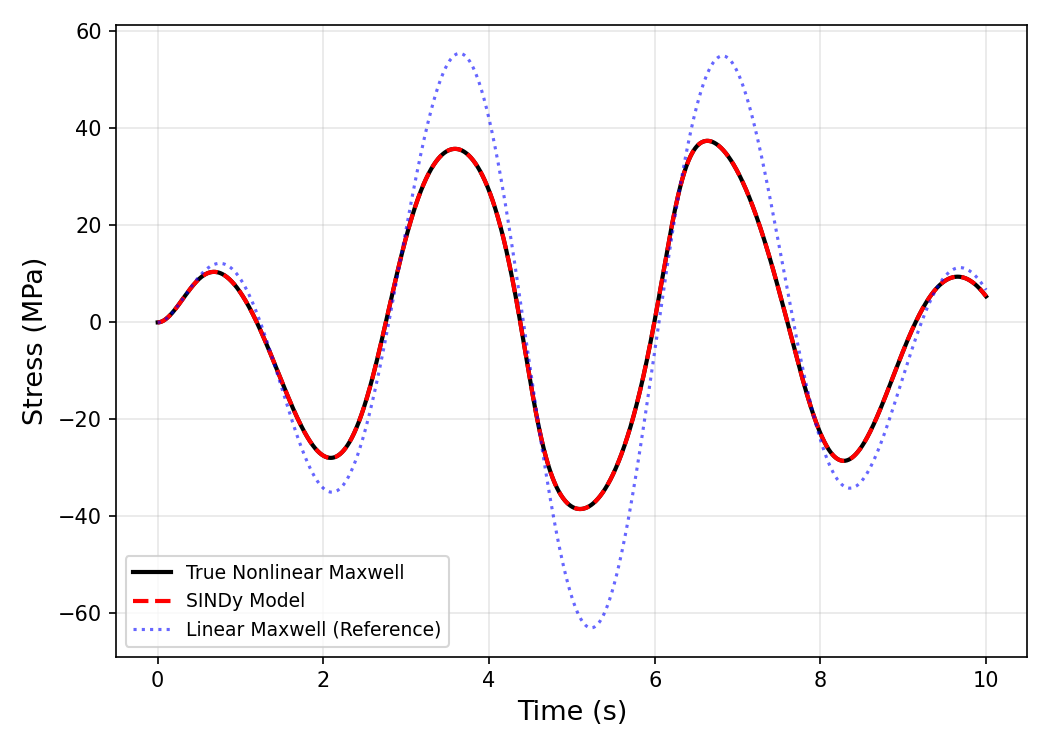
\includegraphics[width=\textwidth]{04_biaxial_Syy_rmse0.0028.png}
        \caption{$S_{yy}$, RMSE $=0.0028$ MPa.}
    \end{subfigure}
    \caption{Biaxial tension validation load. \texttt{03\_biaxial\_Sxx\_rmse0.0032.png} / \texttt{04\_biaxial\_Syy\_rmse0.0028.png}.}
\end{figure}

\begin{figure}[htbp]
    \centering
    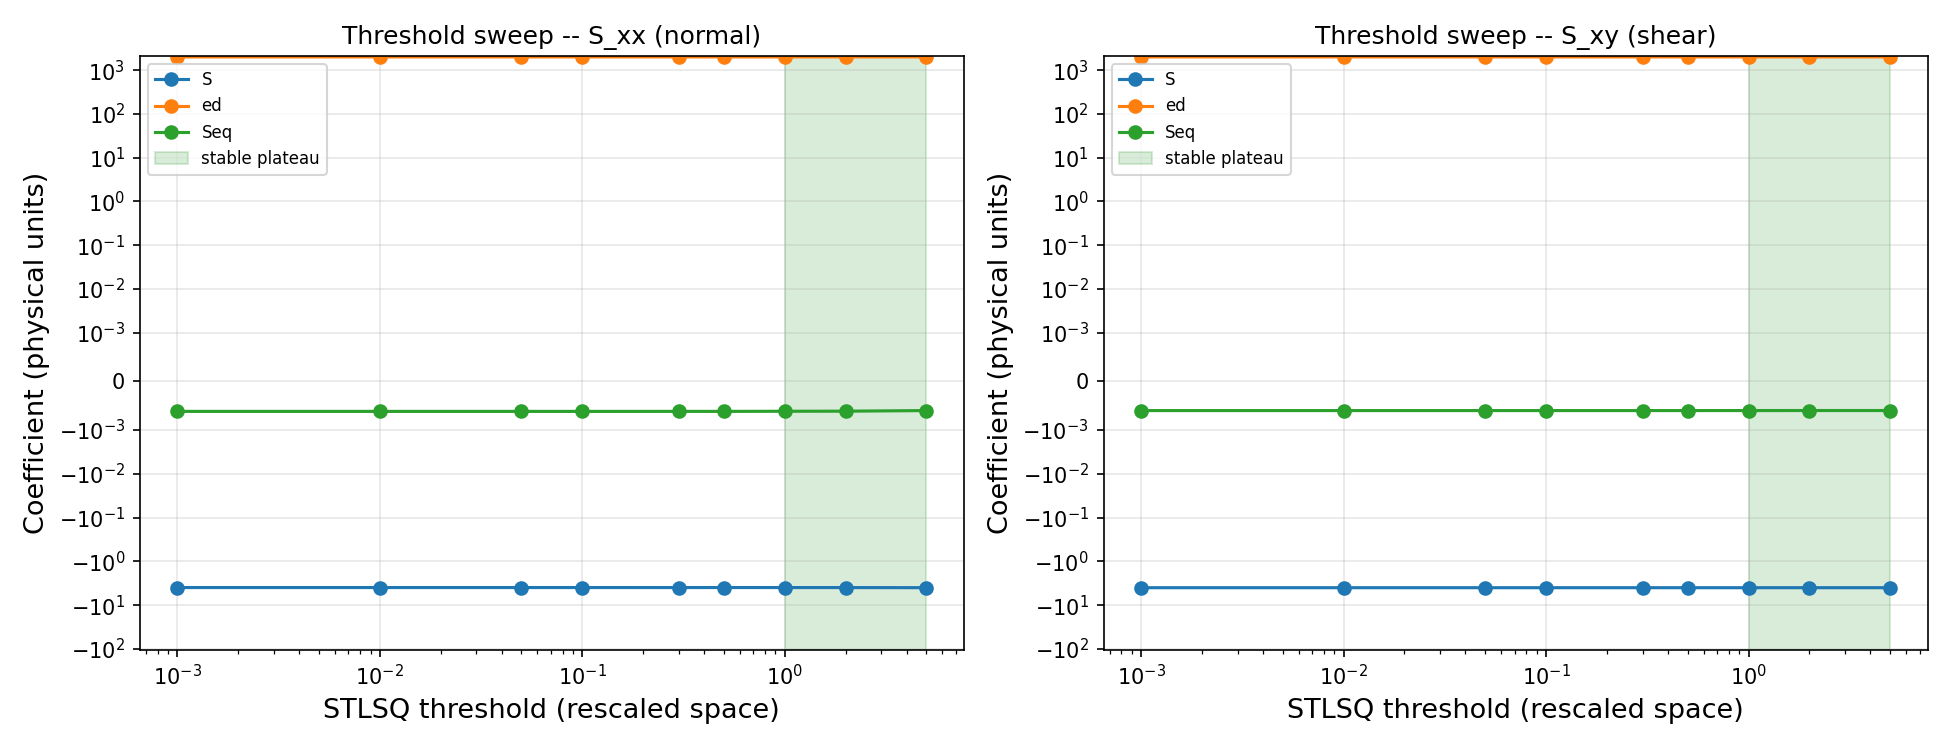
\includegraphics[width=0.95\textwidth]{05_threshold_sensitivity_sweep_degree3_rescaled.png}
    \caption{\texttt{05\_threshold\_sensitivity\_sweep\_degree3\_rescaled.png} -- Coefficient value (physical units, symlog scale) vs. STLSQ threshold (rescaled space, log scale) for the $S$, $\dot\varepsilon$, and $Seq$ terms, for both the normal and shear component fits. All three true terms are flat and nonzero across the green plateau $[1.0, 5.0]$; every other library term (not shown) is zero there. This is the direct visual evidence that rescale--prune--unscale recovers the correct sparsity pattern from a degree-3 library, not a hand-picked single threshold.}
    \label{fig:sweep_3d_degree3}
\end{figure}

\end{document}
